% !TEX program = lualatex
\documentclass[12pt,a4paper]{article}
\usepackage{fontspec}
\setmonofont{Latin Modern Mono}
\usepackage{xcolor}
\usepackage{listings}
\usepackage{geometry}
\usepackage{fancyhdr}
\usepackage{hyperref}
\usepackage{graphicx}
\geometry{margin=1in}
\usepackage{multicol}

% -------------------------------
% SOLUTION TOGGLE
% -------------------------------
\newif\ifshowsolutions
% \showsolutionstrue 
\showsolutionsfalse

% -------------------------------
% Header and Footer Configuration
% -------------------------------
\pagestyle{fancy}
\fancyhf{}
\lhead{Lab Final}
\rhead{CSE 4308: DBMS Lab}
\cfoot{\thepage}
\setlength{\headwidth}{\textwidth}

% -------------------------------
% Code Listing Style
% -------------------------------
\definecolor{codegreen}{rgb}{0,0.6,0}
\definecolor{codegray}{rgb}{0.5,0.5,0.5}
\definecolor{codepurple}{rgb}{0.58,0,0.82}
\definecolor{backcolour}{rgb}{0.95,0.95,0.92}

\lstdefinestyle{mystyle}{
    backgroundcolor=\color{backcolour},
    commentstyle=\color{codegreen},
    keywordstyle=\color{magenta},
    numberstyle=\tiny\color{codegray},
    stringstyle=\color{codepurple},
    basicstyle=\ttfamily\footnotesize,
    breaklines=true,
    captionpos=b,
    keepspaces=true,
    numbers = none,
    numbersep=5pt,
    tabsize=2,
    frame=single,
    columns=fullflexible,
    showspaces=false,
    showstringspaces=false,
    showtabs=false
}

\lstset{style=mystyle}

% Images: found next to this file (local compile_labs.sh) or via the
% lab folder when compiled from the project root (Overleaf).
\graphicspath{{lab_14_final/}}

\begin{document}

% --------------------------------------------------------------
% TITLE PAGE
% --------------------------------------------------------------
\begin{titlepage}
    \centering
    \vspace*{2\baselineskip}

    \rule{14cm}{2pt}\vspace*{-0.8\baselineskip}\vspace*{1.5pt}
    \rule{14cm}{0.5pt}\vspace{2\baselineskip}

    {\Huge\bfseries\scshape Lab Final\par}
    \vspace{3mm}
    {\Large }
    \vspace{3mm}

    \rule{14cm}{0.5pt}\vspace*{-0.7\baselineskip}\vspace{2.5pt}
    \rule{14cm}{2pt}

    \vspace{2\baselineskip}

    {\Large\bfseries CSE 4308\par}
    \vspace{1\baselineskip}
    {\large DATABASE MANAGEMENT SYSTEMS LAB\par}

    \vfill
    {\normalsize Prepared by:\\ Samnun Azfar, Jr. Lecturer, CSE\\ Samia Nawsheen, Jr. Lecturer, CSE\par}
    {\normalsize Academic Year: AY25-26\par}
\end{titlepage}

\newpage

% ==============================================================
\section{Lab Final}

\begin{enumerate}

% ==============================================================
\item List the \texttt{customer\_id}, \texttt{first\_name}, and \texttt{last\_name} of all customers whose \texttt{last\_name} starts with the letter \texttt{'S'}. Order by \texttt{customer\_id}.

\ifshowsolutions
\begin{lstlisting}[language=SQL]
SELECT customer_id, first_name, last_name
FROM customer
WHERE last_name LIKE 'S%'
ORDER BY customer_id;
\end{lstlisting}
\fi


% ==============================================================
\item Find the films that have been rented \textbf{more than 20 times}. 
Show film id, title, and rental count. Order by rental count descending.

\ifshowsolutions
\begin{lstlisting}[language=SQL]
SELECT f.film_id, f.title,
       COUNT(r.rental_id) AS rental_count
FROM film f
JOIN inventory i ON i.film_id = f.film_id
JOIN rental r ON r.inventory_id = i.inventory_id
GROUP BY f.film_id, f.title
HAVING COUNT(r.rental_id) > 20
ORDER BY rental_count DESC, f.film_id;
\end{lstlisting}
\fi


% ==============================================================
\item Find the \textbf{top 10 films} by total revenue (sum of payment.amount). Show film id, title, and total revenue.

\ifshowsolutions
\begin{lstlisting}[language=SQL]
SELECT f.film_id, f.title,
       SUM(p.amount) AS total_revenue
FROM film f
JOIN inventory i ON i.film_id = f.film_id
JOIN rental r ON r.inventory_id = i.inventory_id
JOIN payment p ON p.rental_id = r.rental_id
GROUP BY f.film_id, f.title
ORDER BY total_revenue DESC, f.film_id
LIMIT 10;
\end{lstlisting}
\fi

% ==============================================================
\item Show each staff member and the \textbf{number of rentals they handled}. Order by rental count descending.

\ifshowsolutions
\begin{lstlisting}[language=SQL]
SELECT s.staff_id, s.first_name, s.last_name,
       COUNT(r.rental_id) AS rentals_handled
FROM staff s
LEFT JOIN rental r ON r.staff_id = s.staff_id
GROUP BY s.staff_id, s.first_name, s.last_name
ORDER BY rentals_handled DESC, s.staff_id;
\end{lstlisting}
\fi

% ==============================================================
\item Write an anonymous block that prints all customers from store 1 whose \texttt{active} status is 0. Print customer id and full name using a loop.

\ifshowsolutions
\begin{lstlisting}[language=SQL]
DO $$
DECLARE
    rec RECORD;
BEGIN
    FOR rec IN
        SELECT customer_id, first_name, last_name
        FROM customer
        WHERE store_id = 1 AND active = 0
        ORDER BY customer_id
    LOOP
        RAISE NOTICE 'Inactive customer: ID=% Name=% %',
            rec.customer_id, rec.first_name, rec.last_name;
    END LOOP;
END $$;
\end{lstlisting}
\fi

% ==============================================================
\item Write an anonymous block that takes a film id (e.g., 1) and prints:
(i) the film title,
(ii) the number of times it was rented, and
(iii) the total revenue from that film.

\ifshowsolutions
\begin{lstlisting}[language=SQL]
DO $$
DECLARE
    v_film_id INT := 1;
    v_title TEXT;
    v_rentals INT;
    v_revenue NUMERIC;
BEGIN
    SELECT title INTO v_title
    FROM film
    WHERE film_id = v_film_id;

    IF NOT FOUND THEN
        RAISE NOTICE 'Film id % not found', v_film_id;
        RETURN;
    END IF;

    SELECT COUNT(r.rental_id),
           COALESCE(SUM(p.amount),0)
    INTO v_rentals, v_revenue
    FROM inventory i
    JOIN rental r ON r.inventory_id = i.inventory_id
    LEFT JOIN payment p ON p.rental_id = r.rental_id
    WHERE i.film_id = v_film_id;

    RAISE NOTICE 'Film: % (id=%), Rentals=%, Revenue=%',
        v_title, v_film_id, v_rentals, v_revenue;
END $$;
\end{lstlisting}
\fi

\item Write an anonymous block that prints the \textbf{top 5 customers} by total spending. Print customer id, full name, and total spending using a loop.

\ifshowsolutions
\begin{lstlisting}[language=SQL]
DO $$
DECLARE
    rec RECORD;
    i INT := 0;
BEGIN
    FOR rec IN
        SELECT c.customer_id, c.first_name, c.last_name,
               SUM(p.amount) AS total_spent
        FROM customer c
        JOIN payment p ON p.customer_id = c.customer_id
        GROUP BY c.customer_id, c.first_name, c.last_name
        ORDER BY total_spent DESC, c.customer_id
    LOOP
        i := i + 1;
        EXIT WHEN i > 5;

        RAISE NOTICE '%) Customer %: % % (Total=%)',
            i, rec.customer_id, rec.first_name, rec.last_name, rec.total_spent;
    END LOOP;
END $$;
\end{lstlisting}
\fi

% ==============================================================
\item Create a function that takes a film ID and a store ID and returns how many copies of that film exist in that store and how many are currently available.

\ifshowsolutions
\begin{lstlisting}[language=SQL]
CREATE OR REPLACE FUNCTION film_availability(p_film_id INT, p_store_id INT)
RETURNS TABLE(total_copies INT, available_copies INT)
LANGUAGE plpgsql
AS $$
DECLARE
    rented_copies INT;
BEGIN
    SELECT COUNT(*)
    INTO total_copies
    FROM inventory i
    WHERE i.film_id = p_film_id
      AND i.store_id = p_store_id;

    SELECT COUNT(DISTINCT r.inventory_id)
    INTO rented_copies
    FROM rental r
    JOIN inventory i ON i.inventory_id = r.inventory_id
    WHERE i.film_id = p_film_id
      AND i.store_id = p_store_id
      AND r.return_date IS NULL;

    available_copies := total_copies - rented_copies;

    RETURN QUERY SELECT total_copies, available_copies;
END;
$$;
-- Invocation (example)
SELECT * FROM film_availability(1, 1);
\end{lstlisting}
\fi

% % ==============================================================
% \item Create a function that returns the total revenue collected by a staff member within a date range (inclusive). Return 0 if no revenue.

% \ifshowsolutions
% \begin{lstlisting}[language=SQL]
% CREATE OR REPLACE FUNCTION staff_revenue(p_staff_id INT, p_from DATE, p_to DATE)
% RETURNS NUMERIC
% LANGUAGE plpgsql
% AS $$
% DECLARE
%     v_total NUMERIC;
% BEGIN
%     SELECT COALESCE(SUM(amount),0)
%     INTO v_total
%     FROM payment
%     WHERE staff_id = p_staff_id
%       AND payment_date::date BETWEEN p_from AND p_to;

%     RETURN v_total;
% END;
% $$;

% -- Invocation (example)
% SELECT staff_revenue(1, '2007-02-01', '2007-05-31');

% \end{lstlisting}
% \fi
% ==============================================================
\item Create a function \texttt{film\_revenue\_range} that returns the total revenue earned by a given film within a given date range.
\ifshowsolutions
\begin{lstlisting}[language=SQL]
CREATE OR REPLACE FUNCTION film_revenue_range(
    p_film_id INT,
    p_from DATE,
    p_to DATE
)
RETURNS NUMERIC
LANGUAGE plpgsql
AS $$
DECLARE
    v_total NUMERIC;
BEGIN
    SELECT COALESCE(SUM(p.amount), 0)
    INTO v_total
    FROM inventory i
    JOIN rental r ON r.inventory_id = i.inventory_id
    JOIN payment p ON p.rental_id = r.rental_id
    WHERE i.film_id = p_film_id
      AND p.payment_date::date BETWEEN p_from AND p_to;

    RETURN v_total;
END;
$$;
-- Invocation (example)
SELECT film_revenue_range(1, '2007-02-14', '2007-05-14');
\end{lstlisting}
\fi

% ==============================================================
\item Create a procedure that takes a rental ID and sets \texttt{return\_date = NOW()} for that rental only if return\_date is currently NULL. If it is already returned, raise a notice and do nothing. If rental id does not exist, raise an exception.

\ifshowsolutions
\begin{lstlisting}[language=SQL]
CREATE OR REPLACE PROCEDURE mark_returned(p_rental_id INT)
LANGUAGE plpgsql
AS $$
DECLARE
    v_current_return TIMESTAMP;
BEGIN
    SELECT return_date
    INTO v_current_return
    FROM rental
    WHERE rental_id = p_rental_id;

    IF NOT FOUND THEN
        RAISE EXCEPTION 'Rental id % not found', p_rental_id;
    END IF;

    IF v_current_return IS NOT NULL THEN
        RAISE NOTICE 'Rental % already returned at %', p_rental_id, v_current_return;
        RETURN;
    END IF;

    UPDATE rental
    SET return_date = NOW()
    WHERE rental_id = p_rental_id;

    RAISE NOTICE 'Rental % marked as returned', p_rental_id;
END;
$$;

-- Invocation (example)
CALL mark_returned(1);
\end{lstlisting}
\fi

% ==============================================================




\end{enumerate}
\newpage
\section{ER Diagram}
\begin{figure}[h]
        \centering
        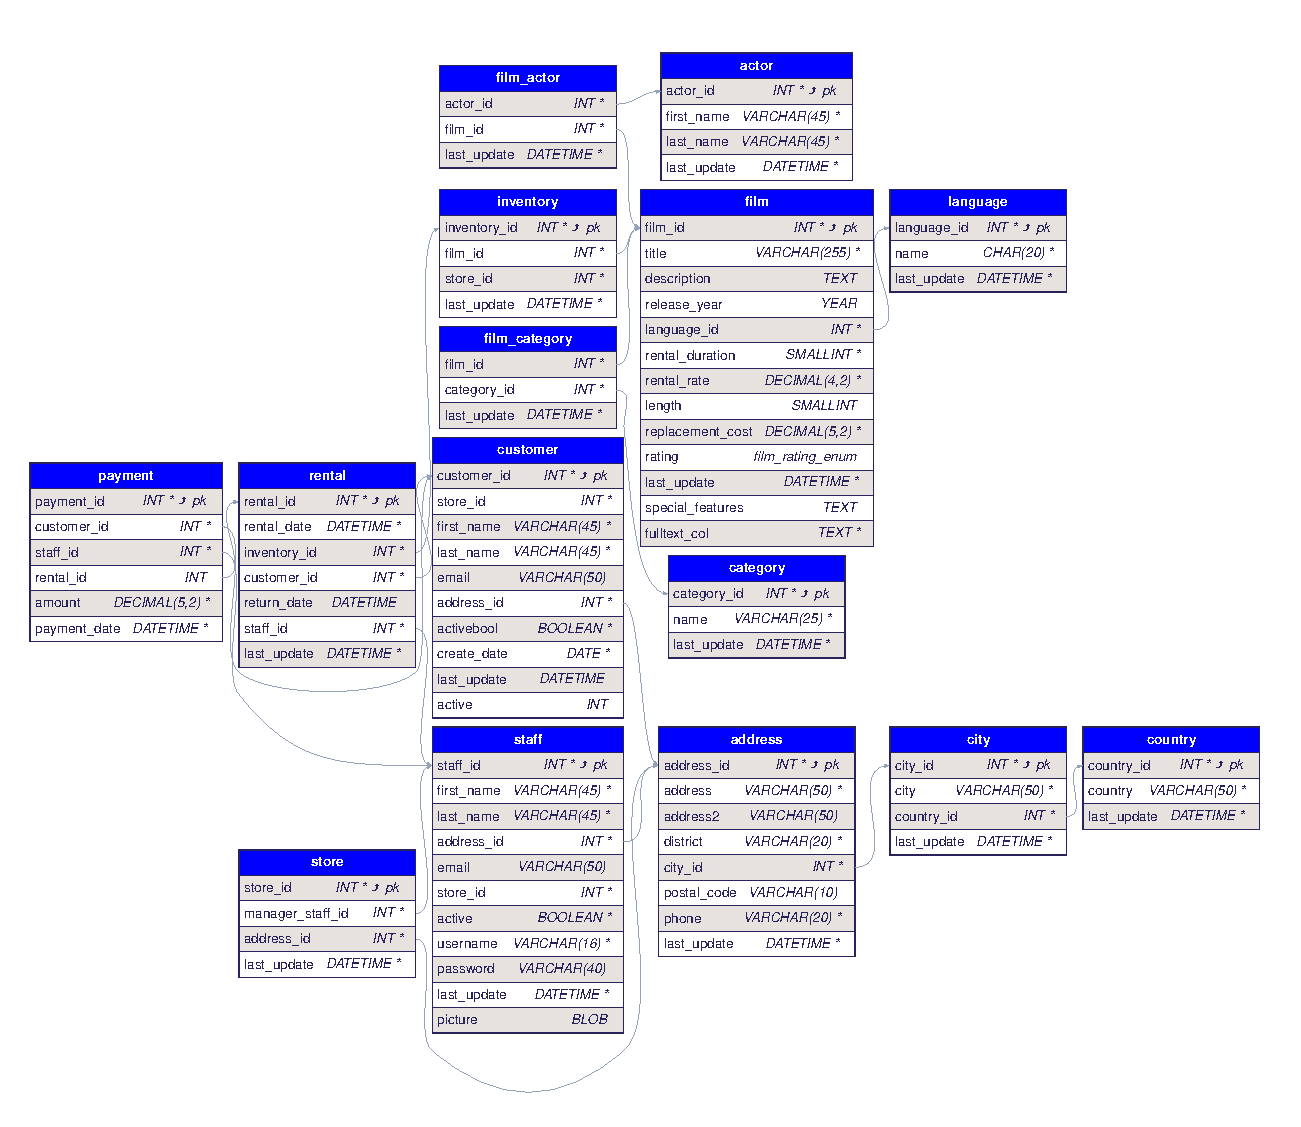
\includegraphics[width=\textheight, height=\textwidth, keepaspectratio, angle=90]{lab_14_schema_cropped.pdf}
\end{figure}
\end{document}